% !TEX root = main.tex

\section{计算机网络概述}
计算机网络将终端设备连接起来并可以传输数据。

\subsection{网络连接方式}
\begin{enumerate}
\item 直接连接的网络(直连网)
\begin{itemize}
\item \underline{点对点(point-to-point)网络}:包括专用介质(dedicated medium)、节点/主机
\begin{itemize}
	\item 单向(simplex):如广播、电视
	\item 半双工(half duplex):异步双向,如对讲机
	\item 全双工(full duplex):同步双向,如电话
\end{itemize}
\item \underline{多路访问(multiple access)网络}:共享介质(shared medium),会产生碰撞(collision)
\begin{itemize}
	\item 单播(unicast):一对一
	\item 多播(multicast):一对多
	\item 广播(broadcast):一对所有
\end{itemize}
\end{itemize}
\item 间接连接的网络:涉及交换机、路由器
\end{enumerate}

\subsection{因特网}
用路由器或网关(gateway)连接起来构成的网络称为互\textred{连}网络(internetwork)。

因特网/互联网(Internet)是一种互连网络,可以看作是把世界各地的广域网互连的网络,是世界上最大的特定计算机网络,采用\textemph{TCP/IP协议簇}作为通信规则。
\begin{itemize}
	\item 系统域网(System Area Network, SAN):电脑、鼠标、USB
	\item 局域网(Local Area Network, LAN):某一区域内由多台计算机互联成的计算机组,一般是方圆几千米以内,如小型实验室;常用\textemph{多路访问网络}
	\item 城域网(Metropolitan Area Network, MAN)
	\item 广域网(Wide Area Network, WAN):\textemph{因特网}
\end{itemize}

\myhline
因特网设备:
\begin{itemize}
	\item 终端系统/主机(end system):运行网络应用程序,如手机、浏览器
	\item 通信链路(communication link):光纤、铜线、无线电、卫星等
	\item 路由器(router):用于连接多个网络形成更大的网络
\end{itemize}

\myhline
因特网的组成:ISP(Internet Service Provider)
\begin{itemize}
	\item 网络边界(network edge):主机及网络程序,终端设备可以通过本地ISP或区域ISP连接上互联网
	\item 接入网络/接入网(access network):有线或无线接入,连接订阅者和服务提供商,如WiFi
	\item 网络核心/主干网(core network):顶层ISP(中国电信、中国移动、中国网通),可以连接局部提供商
\end{itemize}

\subsection{网络服务}
通信服务类型:
\begin{itemize}
	\item 可靠/不可靠:会不会丢包/收发是否完全相同,如文件(可靠)/视频(不可靠)
	\item 面向连接/无连接:需不需要建立通信线路,如电话(连接,双方都要在)/寄信、因特网(无连接,对方可能不在)
	\item 有确认/无确认:需不需要确认对方是否收包,因特网不需要
	\item 请求响应/消息流服务:有请求才有响应/一直发消息,如电视
\end{itemize}

因特网是\textemph{数据报服务},\textemph{无连接无确认(尽力服务)}。

\subsection{因特网体系结构}
因特网体系结构包括以下这\textemph{五层},而ISO/OSI(open system interconnection)网络包括七层协议\footnote{也有TCP/IP四层的说法,将物理层和数据链路层合并起来变成物理网络层}:
\begin{itemize}
	\item 应用层:提供对某些专门应用的支持,如\underline{FTP、SMTP、HTTP}
	\item (OSI)表示层(presentationn):提供数据转换服务, 如\underline{加密解密,压缩解压缩,数据格式变换}
	\item (OSI)会话层(session):简化会话实现机制,如\underline{数据流的检查点设置和回滚,多数据流同步}
	\item 传输层:将网络层获得的包在\textemph{进程之间}数据传送(端到端),如\underline{TCP、UDP}
	\item 网络层:\textemph{路由选择},实现在互联网中的数据传送(主机到主机),如\underline{IP协议、路由协议}
	\item 数据链路层:在\textemph{物理网络}中传送\textemph{包}(跳到跳\footnote{一跳(hop)/节点为一个物理设备,即数据链路层只考虑直连网的情况},节点到节点),如\underline{PPP、Ethernet}
	\item 物理层:线上的\textemph{比特}(传送原始比特流)
\end{itemize}
\par 其中\textemph{网络层以下不可靠,以上可靠};防止丢包的机制:\textemph{重发}。
\par 物理层和数据链路层又被称为\underline{物理网络},网络层和传输层被称为\underline{逻辑网络}。

\myhline
协议(protocol):在网络实体(entities)之间传送消息的规则,如消息的格式、收发消息的次序等。

每层传输的数据单元都称为\textemph{包}(packets),都属于某个协议,又被称为\textemph{协议数据单元}(protocol data unit, PDU),包括\textemph{头部/协议控制信息}(potocal control data, PCI)和\textemph{服务数据单元}(service data unit, SDU)两部分。

\begin{minipage}{0.4\linewidth}
\begin{center}
\begin{tikzcd}
\text{应用层Application}\arrow{d}{\text{消息message}}\\
\text{传输层Transport}\arrow{d}{\text{数据段segment}}\\
\text{网络层Network}\arrow{d}{\text{数据报datagram}}\\
\text{链路层Data-link}\arrow{d}{\text{帧frame}}\\
\text{物理层Physical}
\end{tikzcd}
\end{center}
\end{minipage}
\begin{minipage}{0.6\linewidth}
\begin{figure}[H]
	\centering
	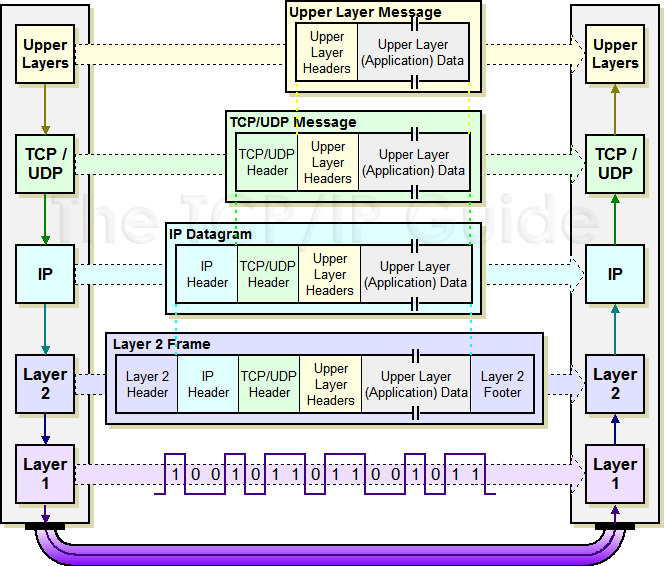
\includegraphics[width=\linewidth]{fig/ipencap.png}
\end{figure}
\end{minipage}

\bigskip
下层把上层通过服务访问点(service access point, SAP)传来的SDU用PCI封装为PDU后传给对等实体(peer entity),即实现相同协议的实体。
同一个互连网络中网络层协议需要相同,链路层协议可以不同。

\myhline
\begin{figure}[H]
	\centering
	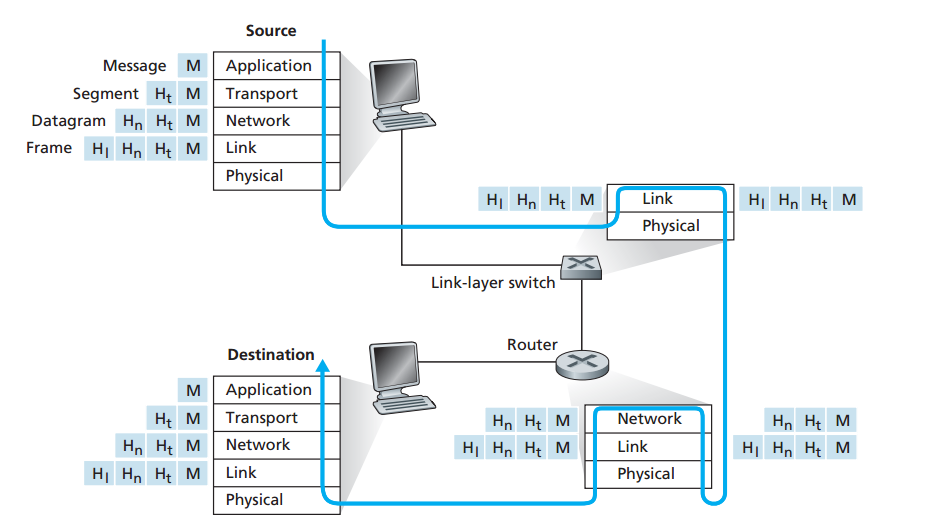
\includegraphics[width=0.8\linewidth]{fig/network-flow.PNG}
	\caption*{协议栈(stack):发送时封装(encaptulation),接收时拆封。}
\end{figure}

\myhline
\begin{figure}[H]
	\centering
	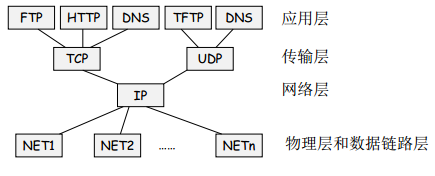
\includegraphics[width=0.5\linewidth]{fig/protocol_family.png}
	\caption*{协议簇(protocol family)}
\end{figure}

\subsection{网络性能分析}
当一个包到达时如果有空闲缓存则排队等待转发,产生延迟(delay);
如果没有空闲缓存,则丢弃该包,造成丢失(loss)。

包交换网络中的延迟主要有以下四点:
\begin{itemize}
	\item 处理(processing)延迟:查路由,存储转发(store-and-forward)的延迟会很大
	\item 排队(queueing)延迟:依赖于路由器的拥塞程度
	\item 发送/传输(transmission)延迟:\[\text{传输延迟}=\text{包长(bits)}/\text{链路带宽(bps, bit per second)}\]
	指从发送第一个包到发送最后一个包的间隔
	\item 传播(propagation)延迟:指对于一个包来说从发送到接收所需的时间
	\[\text{传播延迟}=\text{物理链路长度}/\text{信号传播速度}\]
\end{itemize}

接收延迟与传播延迟重合。
故忽略掉处理、排队延迟,
\[\text{总延迟(从第一个包被发送到最后一个包被接收的时间)}=\text{传播延迟}+\text{发送延迟}\]

\myhline
\par 往返时间(round trip time, RTT):从源主机到目的主机再返回源主机所花的时间
\par 带宽(bandwidth):一条链路或通道可达到的\textemph{最大}数据传输速率(bps)
\par 吞吐量(thoughput):一条链路或通路\textemph{实际}数据传输速率

\begin{example}
	如果一个长度为$3000$字节的文件用一个数据包从源主机通过一段链路传给了一个交换机,然后再通过第二段链路到达目的主机。
	如果在包交换机的延迟为$2ms$,两条链路上的传播延迟都是$2\times 10^8m/s$,带宽都是$1Mbps$,长度都是$6000km$。
	采用以下三种方式,问这个文件在这两台主机之间的总延迟是多少?
	\begin{enumerate}
		\item 交换机采用存储转发方式
		\item 将文件分成10个数据包,且存储转发
		\item 收到一位转发一位
	\end{enumerate}
\end{example}
\begin{analysis}
	\begin{enumerate}
	\item 因采用存储转发技术,先计算一段的延时,最后乘2。
	\begin{itemize}
	\item 一段的传输延时:$3000B\times 8/10^6bps=24$ms
	\item 一段的传播延时:$6000km/(2\times 10^8m/s)=30$ms
	\item 转发延时:$2$ms
	\end{itemize}
	总时长:$(24+30)\times 2+2=110$ms
	\item 类似1,但是总时长是一个包的传输传播转发延迟,加上剩余包的接收/传输延迟,见下表加粗部分
	\begin{center}
		\begin{tabular}{|c|c|c|c|c|c|}\hline
			包1 & \textemph{传输} & \textemph{传播} & \textemph{接收} & & \\\hline
			包2 &  & 传输 & 传播 & \textemph{接收} & \\\hline
			包3 &  &  & 传输 & 传播 & \textemph{接收} \\\hline
		\end{tabular}
	\end{center}
	\begin{itemize}
		\item 一段的传输延时:$300B\times 8/10^6bps=2.4$ms
		\item 一段的传播延时:$30$ms
		\item 转发延时:$2$ms
	\end{itemize}
	总时长:$(2.4+30)\times 2+2+2.4\times 9=88.4$ms
	\item 同1,但是只用计算一段传输延时,因为1位的转发延迟忽略。
	故总时长:$24+30\times 2=84$ms
\end{enumerate}
\end{analysis}